\subsection{题目描述}
\noindent Given \( n+1 \) points \((x_0, y_0), (x_1, y_1), \dots, (x_n, y_n)\), the \( n \)-th order interpolation polynomial using Newton's method is:
\[
P_n(x) = f[x_0] + f[x_1, x_0](x - x_0) + f[x_2, x_1, x_0](x - x_0)(x - x_1) + \cdots + f[x_n, x_{n-1}, \dots, x_0](x - x_0)(x - x_1) \dots (x - x_{n-1})
\]
where \( f[x_i, x_{i-1}, \dots, x_0] \) represents the divided differences. Taking the coefficients from the lower edge of the difference table (i.e., \( f[x_n], f[x_n, x_{n-1}], \dots, f[x_n, \dots, x_0] \)), will this provide higher accuracy for values of \( x \) near \( x_n \)?

\begin{center}
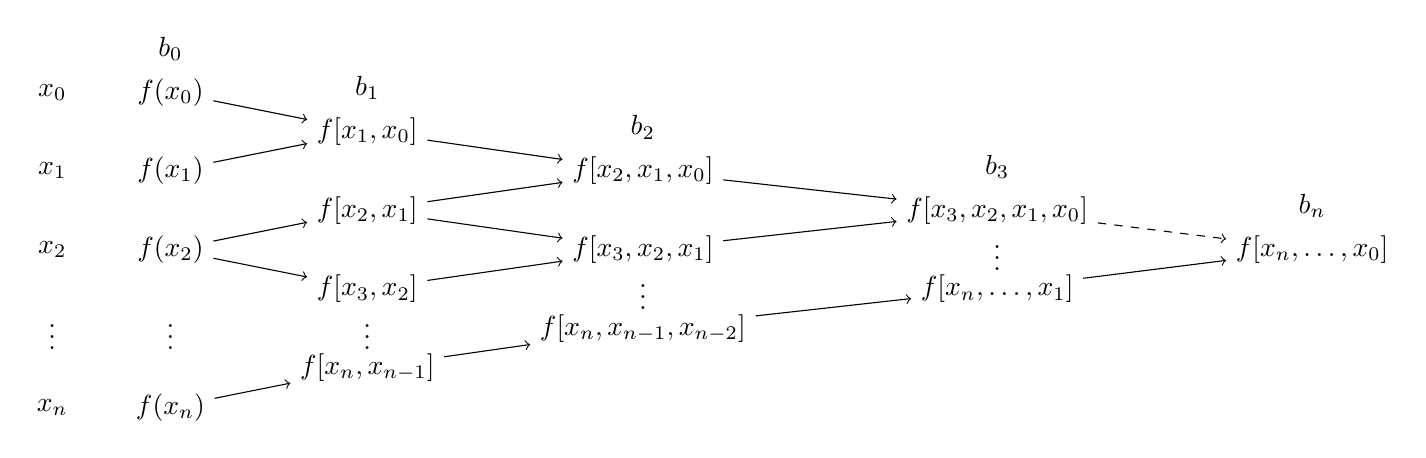
\begin{tikzpicture}
    % Column 1 (x values)
    \node (x0) at (-4, 0) {$x_0$};
    \node (x1) at (-4, -1) {$x_1$};
    \node (x2) at (-4, -2) {$x_2$};
    \node (dots) at (-4, -3) {$\vdots$};
    \node (xn) at (-4, -4) {$x_n$};

    % Column 2 (f(x) values)
    \node (f0) at (-2.5, 0) {$f(x_0)$};
    \node (f1) at (-2.5, -1) {$f(x_1)$};
    \node (f2) at (-2.5, -2) {$f(x_2)$};
    \node (fdots) at (-2.5, -3) {$\vdots$};
    \node (fn) at (-2.5, -4) {$f(x_n)$};

    % Column 3 (f[x1, x0], etc.)
    \node (f10) at (0, -0.5) {$f[x_1, x_0]$};
    \node (f21) at (0, -1.5) {$f[x_2, x_1]$};
    \node (f32) at (0, -2.5) {$f[x_3, x_2]$};
    \node (fdots2) at (0, -3) {$\vdots$};
    \node (fnn1) at (0, -3.5) {$f[x_n, x_{n-1}]$};

    % Column 4 (f[x2, x1, x0], etc.)
    \node (f210) at (3.5, -1) {$f[x_2, x_1, x_0]$};
    \node (f321) at (3.5, -2) {$f[x_3, x_2, x_1]$};
    \node (fdots3) at (3.5, -2.5) {$\vdots$};
    \node (fnnn2) at (3.5, -3) {$f[x_n, x_{n-1}, x_{n-2}]$};

    % Column 5 (f[x3, x2, x1, x0], etc.)
    \node (f3210) at (8, -1.5) {$f[x_3, x_2, x_1, x_0]$};
    \node (fdots4) at (8, -2) {$\vdots$};
    \node (fnnnn3) at (8, -2.5) {$f[x_n, \dots, x_1]$};

    % Column 6 (final term)
    \node (final) at (12, -2) {$f[x_n, \dots, x_0]$};

    % Labels for coefficients
    \node[above=8pt] at (f0) {$b_0$}; % 向上偏移8pt
    \node[above=8pt] at (f10) {$b_1$};
    \node[above=8pt] at (f210) {$b_2$};
    \node[above=8pt] at (f3210) {$b_3$};
    \node[above=8pt] at (final) {$b_n$};

    % Drawing connections with (dashed) lines
    \draw[->] (f0) -- (f10);
    \draw[->] (f10) -- (f210);
    \draw[->] (f210) -- (f3210);
    \draw[dashed, ->] (f3210) -- (final);

    % Drawing vertical solid lines within each column
    \draw[->] (f1) -- (f10);
    \draw[->] (f2) -- (f21);
    \draw[->] (f2) -- (f32);
    \draw[->] (f21) -- (f210);
    \draw[->] (f21) -- (f321);
    \draw[->] (f32) -- (f321);
    \draw[->] (f321) -- (f3210);
    \draw[->] (fn) -- (fnn1);
    \draw[->] (fnn1) -- (fnnn2);
    \draw[->] (fnnn2) -- (fnnnn3);
    \draw[->] (fnnnn3) -- (final);

\end{tikzpicture}
\end{center}

\subsection{程序描述}
原本对于不考虑舍入误差的理想形式,Newton插值与Lagrange插值的结果必定是唯一且等价的,也即通过给定$(n+1)$个节点的$n$阶多项式唯一,这一点可以从Vandermonde行列式
\[
\det \begin{pmatrix}
1 & x_0 & x_0^2 & \cdots & x_0^n \\
1 & x_1 & x_1^2 & \cdots & x_1^n \\
\vdots & \vdots & \vdots & & \vdots \\
1 & x_n & x_n^2 & \cdots & x_n^n
\end{pmatrix} = \prod_{0 \leq i < j \leq n} (x_j - x_i)
\]
非奇异中看出。但实际结果中,我们必须考虑舍入误差,这使得Newton插值的结果可能会依赖于节点的顺序。尤其是在我们使用Horner's Rule(\ref{eq:horner})的时候,显然在节点附近的插值数值稳定性依赖于节点的顺序。本程序使用\ref{sec:problem_1}节中的牛顿插值代码,对两个病态函数\(\mathrm{e}^x\)与\(\sin(100x)\)展开了数值实验。

实验中,我们分别在区间\([-10, 10]\)和\([-0.8, 0.5]\)上等距取25个节点,对两个函数进行顺序与逆序的牛顿插值,并在子图1中展示插值效果,在子图2中对比两者相较于真实函数的相对误差,在子图3中展示逆序插值与顺序插值相对误差的差值。在\(\mathrm{e}^x\)结果中使用了对数坐标轴以更好展示插值效果。
\subsection{实验结果}
\begin{figure}[H]
    \centering
    \includegraphics[width=1.0\textwidth]{Problem_3/figs/exp.png}
    \caption{\(\mathrm{e}^x\)实验结果}
\end{figure}
令人惊奇的是,对于病态函数\(\mathrm{e}^x\),顺序插值的效果始终优于逆序插值(表现为子图2中蓝色虚线始终位于橙色虚线下方,子图3中紫色曲线值始终非负)猜测可能是由于逆序差值的系数在计算初期便受到了较大的舍入误差的影响,而这种影响在Horner's Rule中被逐级放大,最终在传播后半段(子图左侧)逐渐显现。

\begin{figure}[H]
    \centering
    \includegraphics[width=1.0\textwidth]{Problem_3/figs/sin.png}
    \caption{\(\sin(100x)\)实验结果}
\end{figure}

对于高频震荡的病态函数\(\sin(100x)\),逆序差值与顺序差值这对卧龙凤雏,均展现了高达一倍以上的相对误差,相较于\(\mathrm{e}^x\)的结果,更为病态,也符合预期。令人惊喜的是,由于\(\sin(100x)\)本身的对称性与导数有界性,两种差值顺序的优劣对比在区间两端出现了符合预期的差别:在正向传播的末端(子图3右侧),顺序插值的相对误差超过了逆序差值,反之在另一侧,顺序差值结果更优,这符合我们最开始的朴素想法:随着节点的进行,舍入误差的影响逐渐增大,致使区间两侧效果不一,这也提示我们在边界附近应当采集更密的节点,如\ref{sec:problem_1}节中的Chebyshev与Leja节点。